%%% Laboratory	 Notes
%%% Template by Mikhail Klassen, April 2013
%%% Contributions from Sarah Mount, May 2014
\documentclass[a4paper]{tufte-handout}

\newcommand{\workingDate}{\textsc{Fall $|$ 2016}}
\newcommand{\userName}{Cail Daley}
\newcommand{\institution}{Wesleyan University}

\usepackage{aumic_notes}


\usepackage{hyperref}
\usepackage{hypcap}
\hypersetup{
    pdffitwindow=false,            % window fit to page
    pdfstartview={Fit},            % fits width of page to window
    pdftitle={HD_100546_Modeling_Notes},     % document title
    pdfauthor={Cail Daley},         % author name
    pdfsubject={},                 % document topic(s)
    pdfnewwindow=true,             % links in new window
    colorlinks=true,               % coloured links, not boxed
    linkcolor=DarkScarletRed,      % colour of internal links
    citecolor=DarkChameleon,       % colour of links to bibliography
    filecolor=DarkPlum,            % colour of file links
    urlcolor=DarkSkyBlue           % colour of external links
}

\title{AU Mic Notes}
\date{2016}

\begin{document}
\maketitle

%%%%%%%%%%%%%%%%%%%%%%%%%%%%%%%%%%%%%%%%%%%%%%%%%%%%%%%%

\begin{tasks}
    \begin{itemize}
      \item Write up :/
      \item remake aumic\_all
      \item package files nicely for Evan
      \item finish up modeling code, post to github
    \end{itemize}
\end{tasks}

%%%%%%%%%%%%%%%%%%%%%%%%%%%%%%%%%%%%%%%%%%%%%%%%%%%%%%%%

\begin{maybe}
    \begin{itemize}
      \item Make primary modeling code function-based
    \end{itemize}
\end{maybe}

%%%%%%%%%%%%%%%%%%%%%%%%%%%%%%%%%%%%%%%%%%%%%%%%%%%%%%%%

\begin{mer}
    \begin{itemize}
      \item ``fits: insufficient information for antenna table''-- is this a problem?
      \begin{itemize}
        \item I'm pretty sure this only happened when I was getting a $\chi^2$ of four... now that it's back to one, this error does not appear.
      \end{itemize}
      \item $\chi^2$ is back to 1-- changing coordinates only affects $\chi^2$ by 0.001 or less, so whatever the problem was it was not coordinates
    \end{itemize}

\end{mer}
%%%%%%%%%%%%%%%%%%%%%%%%%%%%%%%%%%%%%%%%%%%%%%%%%%%%%%%%

\newday{13 January 2017}
AU Mic was observed on three nights: 18 August 2014, 26 March 2014, and 24 June 2015.

\hrulefill
%%%%%%%%%%%%%%%%%%%%%%%%%%%%%%%%%%%%%%%%%%%%%%%%%%%%%%%%

\newday{13 January 2017}

Cleaning up Modeling\_Code, and deleted the following--noting it here in case it's needed later.
\noindent 18aug2014 phasecenter='J2000 20h45m09.854710s -031d20m32.52034s'\
24jun2015 phasecenter='J2000 20h45m09.867700s -31d20m32.89000s'\
26mar2014 phasecenter='J2000 20h45m09.844300s -031d20m32.36000s'\


\hrulefill
%%%%%%%%%%%%%%%%%%%%%%%%%%%%%%%%%%%%%%%%%%%%%%%%%%%%%%%%

\newday{11 January 2017}

Quite accidentally, Meredith and I stumbled upon what was responsible for corrupting the visibilities. In order to ascertain how long the observations were on the flare date we plotted time vs. amplitude using uvplt (\textit{uvplt vis=24jun2015\_aumic1\_spw3.corrected\_weights.vis/ axis=time,amp device=/xs options=nobase}) and found that the last observation time window had become wonky, as seen in Figure \ref{fig:bad_vis}. To fix this, I wrote a function to remove the last observation timewindow using the miriad command uvaver. The visibility file that uvaver spits out has one fewer index than the input file, so I added a conditional to my $\chi^2$-finding function to accommodate this.

\begin{figure}[!ht]
  \label{fig:bad_vis}
  \centering
  \caption{Amplitude as a function of time for the file with the worst $\chi^2$. The final observation window is clearly corrupted.}

  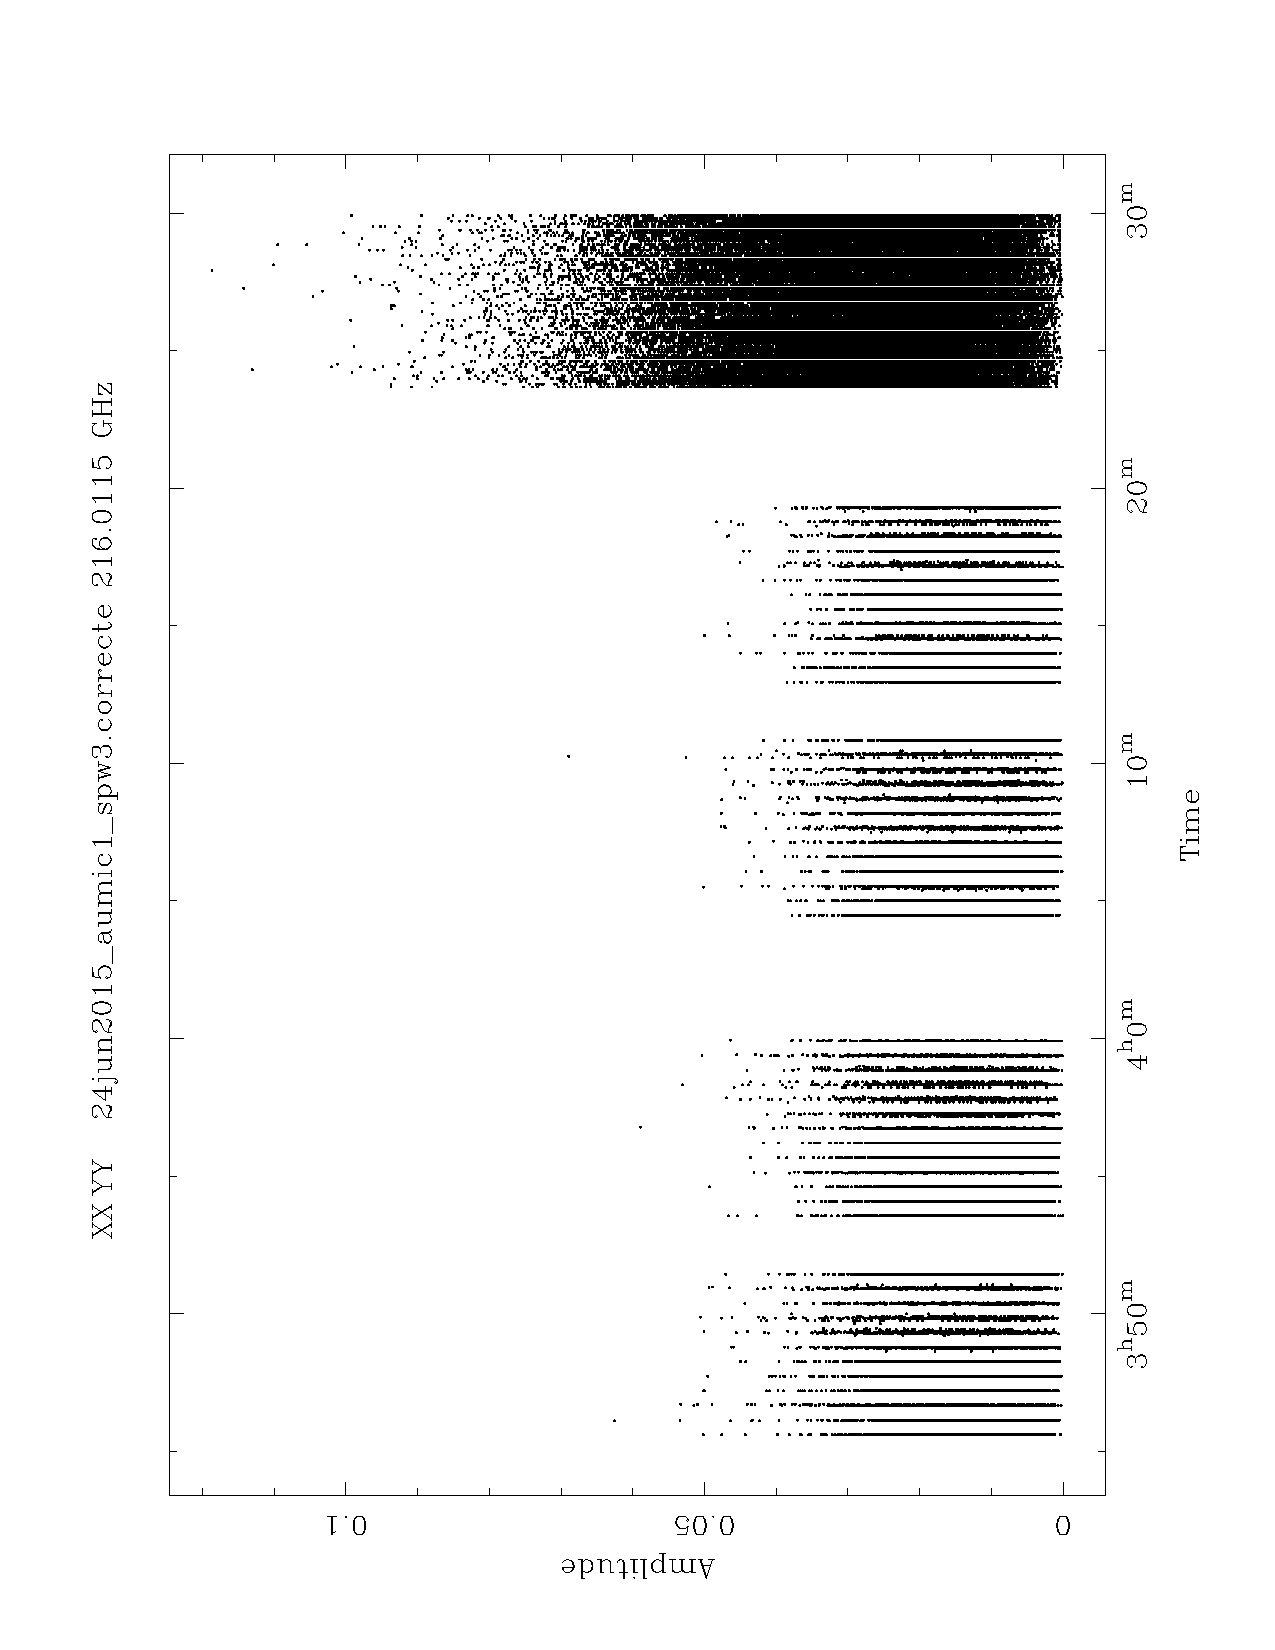
\includegraphics[width=\textwidth, angle=-90]{bad_vis_plot}
\end{figure}


\hrulefill
%%%%%%%%%%%%%%%%%%%%%%%%%%%%%%%%%%%%%%%%%%%%%%%%%%%%%%%%

\newday{18 November 2016}

\paragraph{Weights} \ \\
While looking at Kevin's weight correction code, Meredith and I realized that the code only calculates the weights for the \textit{real} component of the visibilities, and does not calculate the imaginary weights. As such, I was applying the real weights to both the real and imaginary visiblities to obtain the $\chi^2$ for my models. This is a decent approximation assuming that the real weights are roughly the same as the imaginary weights, i.e. \textbf{that the real dispersion is roughly the same as the imaginary dispersion}. However, plotting the real weight vs. the imaginary weights implies that this is not the case, and regardless some accuracy is lost using this approximation. Instead, we are calculating the total weight for each point as
\begin{align}
  \label{weight}
  wt_{tot} = \sqrt{wt_{real}wt_{imaginary}}
\end{align}
and inserting the total weights into both the xx and yy polarization columns of each data file.\\
When calculating the corrected weights for each file using the method described above, the code prints the mean absolute difference between the real and imaginary weights, defined as
\begin{align*}
  \mu_{diff} = \frac{\sum |wt_{real}-wt_{imaginary}|}{N}
\end{align*}
The values for $\mu_{diff}$, as well as $\chi^2$s calculated with the corrected weights, are tabulated below.

\begin{tabular}{lrr}
\toprule
File &  Reduced $\chi^2$ & $\mu_{diff}$ \\
\midrule
18aug2015\_spw0 &          2.04 & \num{2777.94} \\
18aug2015\_spw1 &          2.04 & 3262.7 \\
18aug2015\_spw2 &          2.04 & 3354.83 \\
18aug2015\_spw3 &          2.05 & 3136.28 \\
\textbf{24jun2015\_spw0} &          2.12 & \num{1.04171e+06} \\
24jun2015\_spw1 &          1.99 & 963318.0 \\
24jun2015\_spw2 &          2.01 & \num{1.26727e+06} \\
\textbf{24jun2015\_spw3} &         12.18 & \num{2.39607e+08} \\
26mar2014\_spw0 &          2.07 & 4755.47 \\
26mar2014\_spw1 &          2.07 & 5064.5 \\
26mar2014\_spw2 &          2.06 & 5180.01 \\
26mar2014\_spw3 &          2.07 & 4431.92 \\
\bottomrule
\end{tabular}

Using Equation \ref{weight} reduced the reduced $\chi^2$s for the bad spectral windows--this implies that the previously un-included imaginary weights tend to be smaller than the real weights. Kevin's weight correcting code also took about a factor of ten longer to run for the June date than for either of the other two.

\hrulefill
%%%%%%%%%%%%%%%%%%%%%%%%%%%%%%%%%%%%%%%%%%%%%%%%%%%%%%%%
\newday{1 November 2016}

\begin{itemize}
  \item Made sure that Modeling\_Code\_check.py deletes existing .vis files before it remakes them to avoid overwrite failure.
  \item Began setting up check code to do the splitting through miriad, rather than CASA-- hopefully I can use the weights created by Kevin's code for the miriad-split visibilities.
\end{itemize}


\hrulefill
%%%%%%%%%%%%%%%%%%%%%%%%%%%%%%%%%%%%%%%%%%%%%%%%%%%%%%%%
\newday{25 October 2016}

Created a new directory in AU\_Mic titled ``fixing\_spws'' to hold things related to fixing bad spws.\\
\indent Created a specialized version of my modeling code, Modeling\_Code\_check.py, to check $\chi^2$ for different spw splits.

\begin{itemize}
  \item Splitting 24 Jun spws 2 and 3 (one good spw and one bad one) by time to compare $\chi^2$
  \item NOTE: Can just use exportuvfits to split
\end{itemize}


\hrulefill
%%%%%%%%%%%%%%%%%%%%%%%%%%%%%%%%%%%%%%%%%%%%%%%%%%%%%%%%

\bibliographystyle{unsrt}
\bibliography{aumic_notes}

\end{document}
